\documentclass[10pt]{article}
\usepackage[a4paper,margin=18mm]{geometry}
\usepackage{amsmath,amssymb,booktabs,array,enumitem}
\usepackage[T1]{fontenc}\usepackage{lmodern}
\usepackage{tikz}\usetikzlibrary{shapes.gates.logic.US,positioning,arrows.meta,patterns,calc}
\usepackage[hidelinks]{hyperref}
\setlength{\parindent}{0pt}\setlength{\parskip}{4pt}
\setlength{\emergencystretch}{2em}
\newcommand{\VDD}{V_{DD}}
\newcommand{\mos}[4]{\begin{scope}[shift={(#1,#2)}]
\draw (0,.24)--(0,-.24);\draw (0,.20)--(.25,.20)--(.25,.5);
\draw (0,-.20)--(.25,-.20)--(.25,-.5);\draw (-.16,.23)--(-.16,-.23);
\ifnum#4=1\draw (-.26,0) circle (.06);\draw (-.75,0)--(-.32,0);\else\draw (-.75,0)--(-.16,0);\fi
\node[anchor=east,font=\scriptsize] at (-.76,0) {$#3$};\end{scope}}
\newcommand{\ground}[2]{\draw (#1,#2)--(#1,{#2-.12});\draw ({#1-.17},{#2-.12})--({#1+.17},{#2-.12});\draw ({#1-.11},{#2-.20})--({#1+.11},{#2-.20});}
\newcommand{\rail}[3]{\draw (#1,#2)--(#1,{#2+.14});\node[above,font=\scriptsize] at (#1,{#2+.14}) {$#3$};}

\newcommand{\hmos}[4]{\begin{scope}[shift={(#1,#2)}]
\draw(-.24,0)--(.24,0);\draw(-.2,0)--(-.2,-.25)--(-.5,-.25);\draw(.2,0)--(.2,-.25)--(.5,-.25);
\draw(-.23,.16)--(.23,.16);
\ifnum#4=1\draw(0,.26)circle(.06);\draw(0,.32)--(0,.75);\else\draw(0,.16)--(0,.75);\fi
\node[below,font=\scriptsize]at(0,-.32){#3};\end{scope}}
\newcommand{\mosvt}[5]{\mos{#1}{#2}{#3}{#4}\ifnum#5=1\draw[line width=1.1pt]({#1-.16},{#2-.23})--({#1-.16},{#2+.23});\fi}\begin{document}
\begin{center}{\large\bfseries Fall 2011 Midterm -- Independently Derived Solutions}\end{center}
\textbf{Scope.} All six questions are retained. Printed question totals sum to 110 points; Q5's 5+5+5+5 subparts sum to 20, as printed. No matching student solution set was found. Original formulas and approximations are retained with explicit physical/model limits. The faint Figure 3 bus junction is reconstructed as connected to VDD, as the user expressly selected.

\textbf{1. Short answers and CMOS realization.}
\begin{enumerate}[label=(\alph*),leftmargin=7mm,itemsep=4pt]
\item Local pattern density affects chemical-mechanical polishing and process uniformity. Density rules and suitable dummy fill reduce dishing, erosion and thickness variation, improving manufacturability and electrical consistency.
\item During plasma processing, a long floating conductor connected to a small MOS gate can collect charge. The resulting gate-oxide stress can damage the oxide; antenna ratio limits, suitable layer jumps or protection diodes reduce the risk.
\item The pull-down realizes $xy+w(u+v)$; its complementary pull-up realizes $(\bar x+\bar y)(\bar w+\bar u\bar v)$. The following complete named-terminal MOS schematic has five NMOS and five PMOS. Repeated terminal names are connected nets.
\begin{center}\begin{tikzpicture}[x=.8cm,y=.82cm,font=\scriptsize]
\mos{0}{0.0}{x}{0}\node[right]at(0.45,0.45){$\mathrm{Nx}$};\node[above]at(0.25,0.5){$f$};\node[below]at(0.25,-0.5){$n1$};
\mos{5}{0.0}{y}{0}\node[right]at(5.45,0.45){$\mathrm{Ny}$};\node[above]at(5.25,0.5){$n1$};\node[below]at(5.25,-0.5){$0$};
\mos{10}{0.0}{w}{0}\node[right]at(10.45,0.45){$\mathrm{Nw}$};\node[above]at(10.25,0.5){$f$};\node[below]at(10.25,-0.5){$n2$};
\mos{0}{-2.25}{u}{0}\node[right]at(0.45,-1.8){$\mathrm{Nu}$};\node[above]at(0.25,-1.75){$n2$};\node[below]at(0.25,-2.75){$0$};
\mos{5}{-2.25}{v}{0}\node[right]at(5.45,-1.8){$\mathrm{Nv}$};\node[above]at(5.25,-1.75){$n2$};\node[below]at(5.25,-2.75){$0$};
\mos{10}{-2.25}{x}{1}\node[right]at(10.45,-1.8){$\mathrm{Px}$};\node[above]at(10.25,-1.75){$V_{DD}$};\node[below]at(10.25,-2.75){$p1$};
\mos{0}{-4.5}{y}{1}\node[right]at(0.45,-4.05){$\mathrm{Py}$};\node[above]at(0.25,-4.0){$V_{DD}$};\node[below]at(0.25,-5.0){$p1$};
\mos{5}{-4.5}{w}{1}\node[right]at(5.45,-4.05){$\mathrm{Pw}$};\node[above]at(5.25,-4.0){$p1$};\node[below]at(5.25,-5.0){$f$};
\mos{10}{-4.5}{u}{1}\node[right]at(10.45,-4.05){$\mathrm{Pu}$};\node[above]at(10.25,-4.0){$p1$};\node[below]at(10.25,-5.0){$p2$};
\mos{0}{-6.75}{v}{1}\node[right]at(0.45,-6.3){$\mathrm{Pv}$};\node[above]at(0.25,-6.25){$p2$};\node[below]at(0.25,-7.25){$f$};
\end{tikzpicture}\end{center}
\item Four properties: full rail-to-rail static output levels; ideally negligible steady-state current apart from leakage; high input impedance; and correct steady-state logic independent of pull-up/pull-down transistor strength ratios (sizing still changes delay and noise margins).
\item In an inverter, PMOS source is VDD, NMOS source is VSS, and both drains join at the output. Both gates join at the input; PMOS body is tied to its well/VDD and NMOS body to substrate/VSS.
\begin{center}\begin{tikzpicture}[x=.8cm,y=.82cm,font=\scriptsize]
\mos{0}{0.0}{A}{1}\node[right]at(0.45,0.45){$\mathrm{P}$};\node[above]at(0.25,0.5){$V_{DD}$};\node[below]at(0.25,-0.5){$Y$};
\mos{5}{0.0}{A}{0}\node[right]at(5.45,0.45){$\mathrm{N}$};\node[above]at(5.25,0.5){$Y$};\node[below]at(5.25,-0.5){$V_{SS}$};
\end{tikzpicture}\\PMOS: upper terminal S, lower D. NMOS: upper D, lower S.\end{center}
\item The output load comprises receiving gate capacitances, output diffusion/junction capacitances, and interconnect capacitance.
\item At $V_{in}=V_{out}=V_{DD}/2$, both devices are saturated under the usual long-channel model. Equal currents require
\[\beta_n(V_{DD}/2-V_{tn})^2=\beta_p(V_{DD}/2-|V_{tp}|)^2.\]
Thus $\beta_p/\beta_n=[(V_{DD}/2-V_{tn})/(V_{DD}/2-|V_{tp}|)]^2$. With equal threshold magnitudes and equal lengths, use $W_p/W_n=\mu_n/\mu_p$ (often about2, but the mobility ratio is not specified in this subquestion).
\end{enumerate}

\newpage\textbf{2. Inverter-chain power and tapering.}
\textbf{(a)} The chain has matched pull-up/pull-down strengths $\beta_i=\{1,2,4,8\}\beta$, since PMOS widths are twice NMOS widths and $\mu_n=2\mu_p$. The four \emph{output} loads are $6C_g,12C_g,24C_g,C_L$; the first inverter's input capacitance is driven by the external source and is not another output load of this chain.
\[\boxed{P_{sw}=fV_{DD}^2(42C_g+C_L).}\]
The first three output slews are each $6\tau_0$ for both edges. Therefore input slews to stages 2,3,4 are each $6\tau_0$; the last output slew $C_L/(8\beta V_{DD})$ does not replace the last \emph{input} slew in the short-circuit expression.
\begin{center}\begin{tabular}{ccccc}\toprule
Stage & PMOS/NMOS widths & $\beta_i/\beta$ & Output load & Input mean slew$/\tau_0$\\\midrule
1&2/1&1&$6C_g$&$(3+2)/2=5/2$\\
2&4/2&2&$12C_g$&6\\
3&8/4&4&$24C_g$&6\\
4&16/8&8&$C_L$&6\\\bottomrule\end{tabular}\end{center}
The printed short-circuit formula assumes equal input edges. For the unequal first edges, use its symmetric linear extension $\tau=(t_r+t_f)/2$; this approximation is explicit. Hence, \emph{using the printed polynomial},
\[
P_{sc}=k\beta(V_{DD}-V_t)^3f\tau_0\left(\frac52+2\cdot6+4\cdot6+8\cdot6\right)
=\boxed{\frac{173}{2}k\beta(V_{DD}-V_t)^3f\tau_0},\qquad P_{dyn}=P_{sw}+P_{sc}.
\]
\textbf{Threshold-convention note.} Simultaneous conduction requires $V_{DD}>V_{tn}+|V_{tp}|$. If the printed $V_t$ denotes that \emph{sum}, its overlap polynomial is consistent as written. If $V_t$ denotes each individual equal threshold magnitude, the ideal-ramp polynomial instead uses $[\max(V_{DD}-2V_t,0)]^3$. Under that convention, replace only the printed polynomial; the chain coefficient 173/2 and load sum remain unchanged. The source does not define this convention. Unequal edge shape and finite load can further change short-circuit current beyond the stated approximation.

\textbf{(b) First input capacitance fixed at the minimum inverter.} If it were free to increase without an input-drive constraint, arbitrarily scaling the whole chain would make the stated optimization ill-posed. With that conventional fixed input and neglected parasitics, a chain of $N$ equally tapered stages with total electrical effort $F=64$ has
\[r=64^{1/N},\qquad D(N)=Nr\,t_d.\]
The continuous stationary ratio is the mathematical Euler number $r=e$. Under the paper's explicit classroom approximation $e\approx2$, use six stages of sizes 1,2,4,8,16,32 times the minimum inverter (both P and N widths); every load ratio is 2, giving $D=12t_d$ and noninverting polarity.
\begin{center}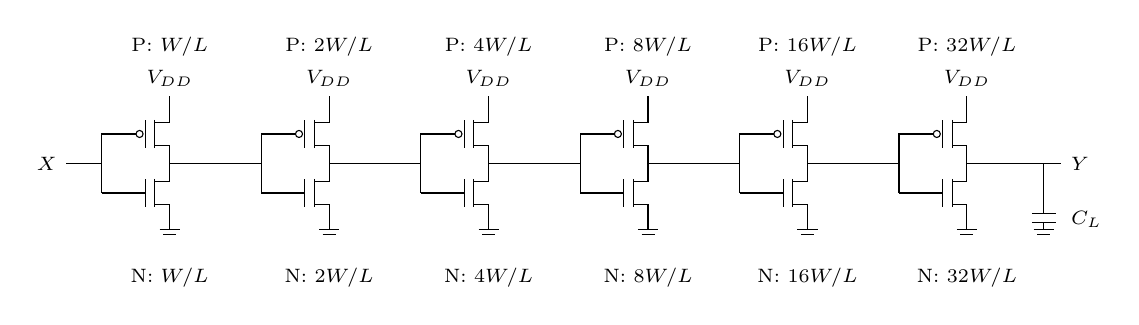
\begin{tikzpicture}[x=.75cm,y=.75cm,font=\scriptsize]
\mos{0.0}{1.5}{}{1}\mos{0.0}{.5}{}{0}\rail{0.25}{2}{V_{DD}}\ground{0.25}{0}\draw(-0.9,.5)--(-0.9,1.5)--(-0.75,1.5);\draw(-0.9,.5)--(-0.75,.5);
\node[above]at(0.25,2.65){P: $W/L$};\node[below]at(0.25,-.6){N: $W/L$};
\draw(-1.5,1)--(-0.9,1)node[pos=0,left]{$X$};
\mos{2.7}{1.5}{}{1}\mos{2.7}{.5}{}{0}\rail{2.95}{2}{V_{DD}}\ground{2.95}{0}\draw(1.8000000000000003,.5)--(1.8000000000000003,1.5)--(1.9500000000000002,1.5);\draw(1.8000000000000003,.5)--(1.9500000000000002,.5);
\node[above]at(2.95,2.65){P: $2W/L$};\node[below]at(2.95,-.6){N: $2W/L$};
\draw(0.25,1)--(1.8000000000000003,1);
\mos{5.4}{1.5}{}{1}\mos{5.4}{.5}{}{0}\rail{5.65}{2}{V_{DD}}\ground{5.65}{0}\draw(4.5,.5)--(4.5,1.5)--(4.65,1.5);\draw(4.5,.5)--(4.65,.5);
\node[above]at(5.65,2.65){P: $4W/L$};\node[below]at(5.65,-.6){N: $4W/L$};
\draw(2.95,1)--(4.5,1);
\mos{8.100000000000001}{1.5}{}{1}\mos{8.100000000000001}{.5}{}{0}\rail{8.350000000000001}{2}{V_{DD}}\ground{8.350000000000001}{0}\draw(7.200000000000001,.5)--(7.200000000000001,1.5)--(7.350000000000001,1.5);\draw(7.200000000000001,.5)--(7.350000000000001,.5);
\node[above]at(8.350000000000001,2.65){P: $8W/L$};\node[below]at(8.350000000000001,-.6){N: $8W/L$};
\draw(5.650000000000001,1)--(7.200000000000001,1);
\mos{10.8}{1.5}{}{1}\mos{10.8}{.5}{}{0}\rail{11.05}{2}{V_{DD}}\ground{11.05}{0}\draw(9.9,.5)--(9.9,1.5)--(10.05,1.5);\draw(9.9,.5)--(10.05,.5);
\node[above]at(11.05,2.65){P: $16W/L$};\node[below]at(11.05,-.6){N: $16W/L$};
\draw(8.350000000000001,1)--(9.9,1);
\mos{13.5}{1.5}{}{1}\mos{13.5}{.5}{}{0}\rail{13.75}{2}{V_{DD}}\ground{13.75}{0}\draw(12.6,.5)--(12.6,1.5)--(12.75,1.5);\draw(12.6,.5)--(12.75,.5);
\node[above]at(13.75,2.65){P: $32W/L$};\node[below]at(13.75,-.6){N: $32W/L$};
\draw(11.05,1)--(12.6,1);
\draw(13.75,1)--(15.35,1)node[right]{$Y$};\draw(15.05,1)--(15.05,.15);\draw(14.85,.15)--(15.25,.15);\draw(14.85,0)--(15.25,0);\ground{15.05}{0}\node[right]at(15.35,.05){$C_L$};
\end{tikzpicture}\end{center}
\textbf{Actual discrete minimum.} Approximating Euler's number by 2 does not change the exact minimum of $N64^{1/N}$. Testing integer stage counts gives $N=4$, $r=2\sqrt2$, and $D=8\sqrt2\,t_d\simeq11.3137t_d$, with widths $1,2\sqrt2,8,16\sqrt2$ times W for both P/N. This four-stage chain also has noninverting polarity. The six-stage result follows the printed approximation; it should not be described as the exact mathematical optimum.
\begin{center}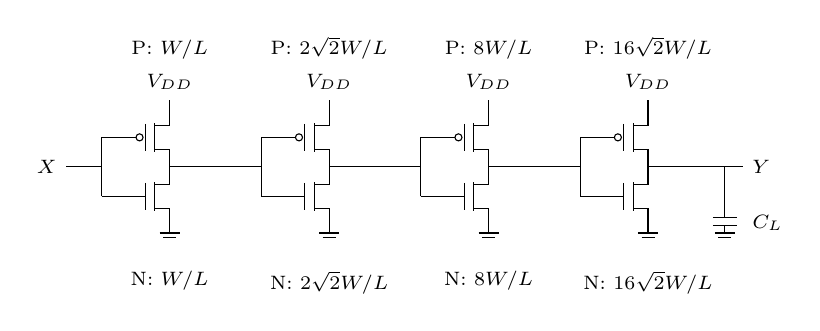
\begin{tikzpicture}[x=.75cm,y=.75cm,font=\scriptsize]
\mos{0.0}{1.5}{}{1}\mos{0.0}{.5}{}{0}\rail{0.25}{2}{V_{DD}}\ground{0.25}{0}\draw(-0.9,.5)--(-0.9,1.5)--(-0.75,1.5);\draw(-0.9,.5)--(-0.75,.5);
\node[above]at(0.25,2.65){P: $W/L$};\node[below]at(0.25,-.6){N: $W/L$};
\draw(-1.5,1)--(-0.9,1)node[pos=0,left]{$X$};
\mos{2.7}{1.5}{}{1}\mos{2.7}{.5}{}{0}\rail{2.95}{2}{V_{DD}}\ground{2.95}{0}\draw(1.8000000000000003,.5)--(1.8000000000000003,1.5)--(1.9500000000000002,1.5);\draw(1.8000000000000003,.5)--(1.9500000000000002,.5);
\node[above]at(2.95,2.65){P: $2\sqrt2W/L$};\node[below]at(2.95,-.6){N: $2\sqrt2W/L$};
\draw(0.25,1)--(1.8000000000000003,1);
\mos{5.4}{1.5}{}{1}\mos{5.4}{.5}{}{0}\rail{5.65}{2}{V_{DD}}\ground{5.65}{0}\draw(4.5,.5)--(4.5,1.5)--(4.65,1.5);\draw(4.5,.5)--(4.65,.5);
\node[above]at(5.65,2.65){P: $8W/L$};\node[below]at(5.65,-.6){N: $8W/L$};
\draw(2.95,1)--(4.5,1);
\mos{8.100000000000001}{1.5}{}{1}\mos{8.100000000000001}{.5}{}{0}\rail{8.350000000000001}{2}{V_{DD}}\ground{8.350000000000001}{0}\draw(7.200000000000001,.5)--(7.200000000000001,1.5)--(7.350000000000001,1.5);\draw(7.200000000000001,.5)--(7.350000000000001,.5);
\node[above]at(8.350000000000001,2.65){P: $16\sqrt2W/L$};\node[below]at(8.350000000000001,-.6){N: $16\sqrt2W/L$};
\draw(5.650000000000001,1)--(7.200000000000001,1);
\draw(8.350000000000001,1)--(9.950000000000001,1)node[right]{$Y$};\draw(9.650000000000002,1)--(9.650000000000002,.15);\draw(9.450000000000001,.15)--(9.850000000000001,.15);\draw(9.450000000000001,0)--(9.850000000000001,0);\ground{9.650000000000002}{0}\node[right]at(9.950000000000001,.05){$C_L$};
\end{tikzpicture}\end{center}

\newpage\textbf{3. Dual-threshold allocation and a real reconvergent glitch.}
\begin{center}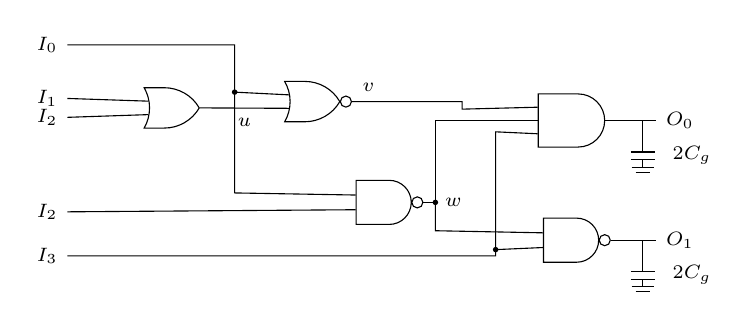
\begin{tikzpicture}[x=.85cm,y=.8cm,font=\scriptsize]
\node[or gate US,draw,logic gate inputs=nn,minimum width=.7cm](u)at(1.2,3){};\node[nor gate US,draw,logic gate inputs=nn,minimum width=.7cm](v)at(3.3,3.1){};\node[nand gate US,draw,logic gate inputs=nn,minimum width=.7cm](w)at(4.4,1.5){};\node[and gate US,draw,logic gate inputs=nnn,minimum width=.7cm](a)at(7.2,2.8){};\node[nand gate US,draw,logic gate inputs=nn,minimum width=.7cm](b)at(7.2,.9){};
\draw(u.input 1)--(-.3,3.15)node[left]{$I_1$};\draw(u.input 2)--(-.3,2.85)node[left]{$I_2$};\draw(u.output)--(v.input 2)node[midway,below]{$u$};\draw(-.3,4)node[left]{$I_0$}--(2.2,4)--(2.2,3.25)--(v.input 1);\draw(2.2,3.25)--(2.2,1.65)--(w.input 1);\fill(2.2,3.25)circle(1pt);\draw(-.3,1.35)node[left]{$I_2$}--(w.input 2);
\draw(v.output)--(5.6,3.1)--(5.6,2.98)--(a.input 1);\node[above]at(4.2,3.1){$v$};\draw(w.output)--(5.2,1.5)--(5.2,2.8)--(a.input 2);\draw(5.2,1.5)--(5.2,1.05)--(b.input 1);\fill(5.2,1.5)circle(1pt);\node[right]at(5.2,1.5){$w$};\draw(-.3,.65)node[left]{$I_3$}--(6.1,.65)--(6.1,.75)--(b.input 2);\draw(6.1,.75)--(6.1,2.62)--(a.input 3);\fill(6.1,.75)circle(1pt);
\draw(a.output)--(8.5,2.8)node[right]{$O_0$};\draw(b.output)--(8.5,.9)node[right]{$O_1$};\foreach\y in {2.8,.9}{\draw(8.3,\y)--(8.3,\y-.5);\draw(8.12,\y-.5)--(8.48,\y-.5);\draw(8.12,\y-.62)--(8.48,\y-.62);\ground{8.3}{\y-.62}\node[right]at(8.6,\y-.55){$2C_g$};}\end{tikzpicture}\end{center}
Name the internal gate outputs
\[u=I_1+I_2,\quad v=\overline{I_0+u},\quad w=\overline{I_0I_2},\quad O_0=v w I_3,\quad O_1=\overline{wI_3}.\]
\textbf{(a) A unique minimum-leakage assignment cannot be computed from the supplied data.} The high-$V_T$ delay increase, high/low-$V_T$ leakage currents, output diffusion loads and the intended allowed timing target are not specified. Even given a baseline target, one must optimize state-weighted leakage subject to the delay constraints; ``noncritical means high-$V_T$'' alone is not proof that speed is preserved.

An explicit illustrative RC normalization uses matched unit pull-up/pull-down resistance, each gate input capacitance $C_g$, and zero diffusion/wire capacitance. Its worst-case gate delays are OR2=$2.5$, NOR2=$1.5$, NAND2 at w=$3$, AND3=$4$, and NAND2 at O1=$3$ inverter-delay units, including OR/AND restoring inverters. This gives paths of8 units through OR--NOR--AND,7 through w--AND, and6 through w--O1. The reference structural target is8 units.

Keep OR, NOR and AND critical-path devices low-$V_T$. A \emph{conditional} illustrative allocation can make both w and O1 NAND gates high-$V_T$ if their extra delays $\Delta_w,\Delta_1$ satisfy
\[\boxed{\Delta_w\leq1,\qquad\Delta_w+\Delta_1\leq2}\]
and all other path constraints hold. If either condition fails, the corresponding devices need low-$V_T$ or a different allocation. The following transistor-level realization explicitly implements the original gate network; L=low-$V_T$, H*=high-$V_T$ \emph{only under those conditions}. It is a feasible conditional example, not an invented global leakage optimum.
\newpage\begin{center}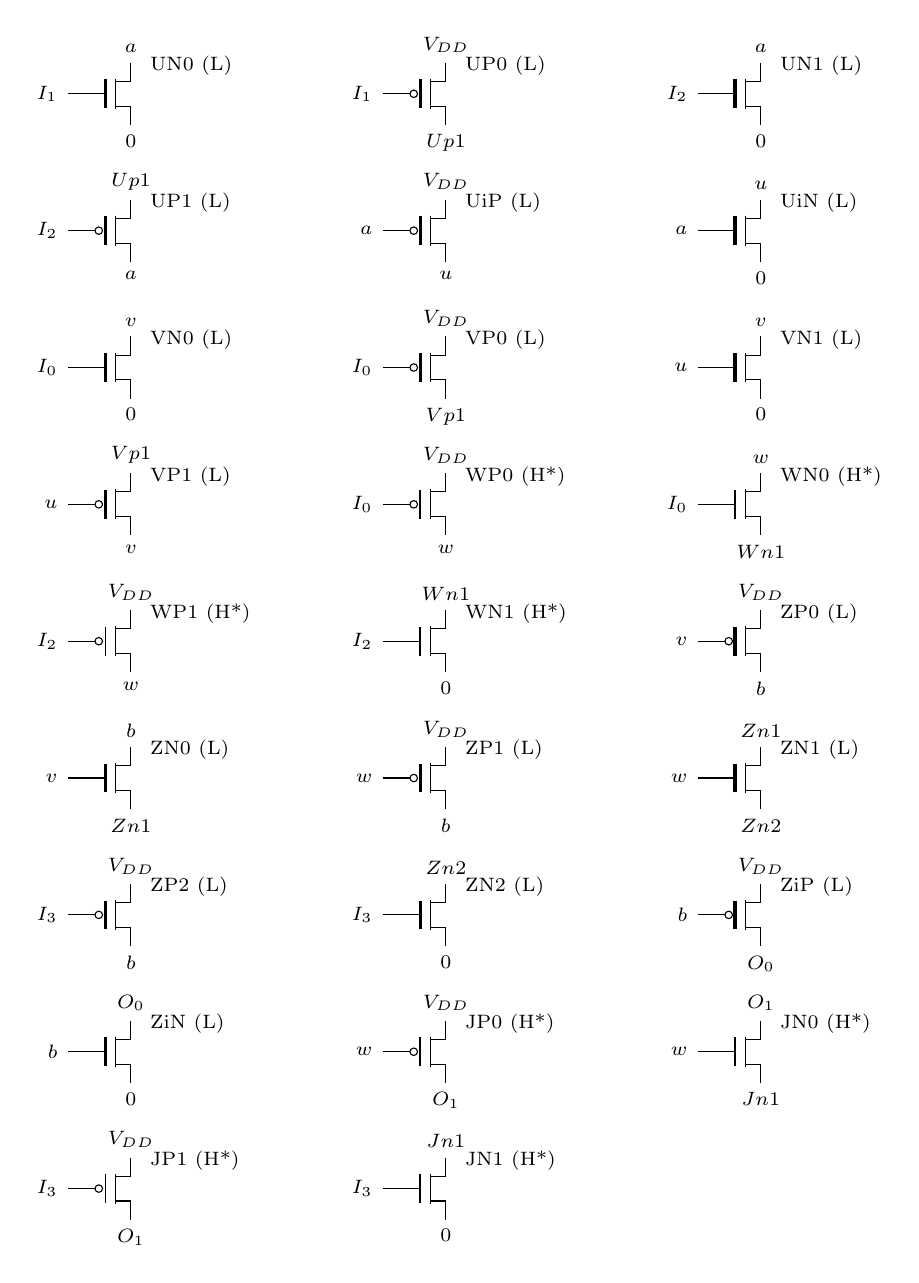
\begin{tikzpicture}[x=.8cm,y=.79cm,font=\scriptsize]
\mosvt{0}{0.0}{I_1}{0}{1}\node[right]at(0.4,0.45){$\mathrm{UN0}$ (L)};\node[above]at(0.25,0.5){$a$};\node[below]at(0.25,-0.5){$0$};
\mosvt{5}{0.0}{I_1}{1}{1}\node[right]at(5.4,0.45){$\mathrm{UP0}$ (L)};\node[above]at(5.25,0.5){$V_{DD}$};\node[below]at(5.25,-0.5){$Up1$};
\mosvt{10}{0.0}{I_2}{0}{1}\node[right]at(10.4,0.45){$\mathrm{UN1}$ (L)};\node[above]at(10.25,0.5){$a$};\node[below]at(10.25,-0.5){$0$};
\mosvt{0}{-2.2}{I_2}{1}{1}\node[right]at(0.4,-1.7500000000000002){$\mathrm{UP1}$ (L)};\node[above]at(0.25,-1.7000000000000002){$Up1$};\node[below]at(0.25,-2.7){$a$};
\mosvt{5}{-2.2}{a}{1}{1}\node[right]at(5.4,-1.7500000000000002){$\mathrm{UiP}$ (L)};\node[above]at(5.25,-1.7000000000000002){$V_{DD}$};\node[below]at(5.25,-2.7){$u$};
\mosvt{10}{-2.2}{a}{0}{1}\node[right]at(10.4,-1.7500000000000002){$\mathrm{UiN}$ (L)};\node[above]at(10.25,-1.7000000000000002){$u$};\node[below]at(10.25,-2.7){$0$};
\mosvt{0}{-4.4}{I_0}{0}{1}\node[right]at(0.4,-3.95){$\mathrm{VN0}$ (L)};\node[above]at(0.25,-3.9000000000000004){$v$};\node[below]at(0.25,-4.9){$0$};
\mosvt{5}{-4.4}{I_0}{1}{1}\node[right]at(5.4,-3.95){$\mathrm{VP0}$ (L)};\node[above]at(5.25,-3.9000000000000004){$V_{DD}$};\node[below]at(5.25,-4.9){$Vp1$};
\mosvt{10}{-4.4}{u}{0}{1}\node[right]at(10.4,-3.95){$\mathrm{VN1}$ (L)};\node[above]at(10.25,-3.9000000000000004){$v$};\node[below]at(10.25,-4.9){$0$};
\mosvt{0}{-6.6000000000000005}{u}{1}{1}\node[right]at(0.4,-6.15){$\mathrm{VP1}$ (L)};\node[above]at(0.25,-6.1000000000000005){$Vp1$};\node[below]at(0.25,-7.1000000000000005){$v$};
\mosvt{5}{-6.6000000000000005}{I_0}{1}{0}\node[right]at(5.4,-6.15){$\mathrm{WP0}$ (H*)};\node[above]at(5.25,-6.1000000000000005){$V_{DD}$};\node[below]at(5.25,-7.1000000000000005){$w$};
\mosvt{10}{-6.6000000000000005}{I_0}{0}{0}\node[right]at(10.4,-6.15){$\mathrm{WN0}$ (H*)};\node[above]at(10.25,-6.1000000000000005){$w$};\node[below]at(10.25,-7.1000000000000005){$Wn1$};
\mosvt{0}{-8.8}{I_2}{1}{0}\node[right]at(0.4,-8.350000000000001){$\mathrm{WP1}$ (H*)};\node[above]at(0.25,-8.3){$V_{DD}$};\node[below]at(0.25,-9.3){$w$};
\mosvt{5}{-8.8}{I_2}{0}{0}\node[right]at(5.4,-8.350000000000001){$\mathrm{WN1}$ (H*)};\node[above]at(5.25,-8.3){$Wn1$};\node[below]at(5.25,-9.3){$0$};
\mosvt{10}{-8.8}{v}{1}{1}\node[right]at(10.4,-8.350000000000001){$\mathrm{ZP0}$ (L)};\node[above]at(10.25,-8.3){$V_{DD}$};\node[below]at(10.25,-9.3){$b$};
\mosvt{0}{-11.0}{v}{0}{1}\node[right]at(0.4,-10.55){$\mathrm{ZN0}$ (L)};\node[above]at(0.25,-10.5){$b$};\node[below]at(0.25,-11.5){$Zn1$};
\mosvt{5}{-11.0}{w}{1}{1}\node[right]at(5.4,-10.55){$\mathrm{ZP1}$ (L)};\node[above]at(5.25,-10.5){$V_{DD}$};\node[below]at(5.25,-11.5){$b$};
\mosvt{10}{-11.0}{w}{0}{1}\node[right]at(10.4,-10.55){$\mathrm{ZN1}$ (L)};\node[above]at(10.25,-10.5){$Zn1$};\node[below]at(10.25,-11.5){$Zn2$};
\mosvt{0}{-13.200000000000001}{I_3}{1}{1}\node[right]at(0.4,-12.750000000000002){$\mathrm{ZP2}$ (L)};\node[above]at(0.25,-12.700000000000001){$V_{DD}$};\node[below]at(0.25,-13.700000000000001){$b$};
\mosvt{5}{-13.200000000000001}{I_3}{0}{1}\node[right]at(5.4,-12.750000000000002){$\mathrm{ZN2}$ (L)};\node[above]at(5.25,-12.700000000000001){$Zn2$};\node[below]at(5.25,-13.700000000000001){$0$};
\mosvt{10}{-13.200000000000001}{b}{1}{1}\node[right]at(10.4,-12.750000000000002){$\mathrm{ZiP}$ (L)};\node[above]at(10.25,-12.700000000000001){$V_{DD}$};\node[below]at(10.25,-13.700000000000001){$O_0$};
\mosvt{0}{-15.400000000000002}{b}{0}{1}\node[right]at(0.4,-14.950000000000003){$\mathrm{ZiN}$ (L)};\node[above]at(0.25,-14.900000000000002){$O_0$};\node[below]at(0.25,-15.900000000000002){$0$};
\mosvt{5}{-15.400000000000002}{w}{1}{0}\node[right]at(5.4,-14.950000000000003){$\mathrm{JP0}$ (H*)};\node[above]at(5.25,-14.900000000000002){$V_{DD}$};\node[below]at(5.25,-15.900000000000002){$O_1$};
\mosvt{10}{-15.400000000000002}{w}{0}{0}\node[right]at(10.4,-14.950000000000003){$\mathrm{JN0}$ (H*)};\node[above]at(10.25,-14.900000000000002){$O_1$};\node[below]at(10.25,-15.900000000000002){$Jn1$};
\mosvt{0}{-17.6}{I_3}{1}{0}\node[right]at(0.4,-17.150000000000002){$\mathrm{JP1}$ (H*)};\node[above]at(0.25,-17.1){$V_{DD}$};\node[below]at(0.25,-18.1){$O_1$};
\mosvt{5}{-17.6}{I_3}{0}{0}\node[right]at(5.4,-17.150000000000002){$\mathrm{JN1}$ (H*)};\node[above]at(5.25,-17.1){$Jn1$};\node[below]at(5.25,-18.1){$0$};
\end{tikzpicture}\end{center}
The supplied input sequence leaves u=1 and v=0, so O0 is always 0 in settled states. That permits additional state-specific opportunities, but startup, transient paths and high-$V_T$ leakage/delay data still determine whether they preserve the requested speed. No numeric leakage saving or unique optimum is claimed.

\newpage\textbf{(b) Equal delays do not remove the glitch.} Let each drawn logic gate have delay $d$, with simultaneous primary-input changes and input dwell time sufficient for settling. In the transition $1100\to1011$, w changes $1\to 0$ after $d$, while I3 changes $0\to1$ immediately. The final O1 NAND first sees $(w,I3)=(1,1)$ and falls at $d$; it then sees $(0,1)$ and rises at $2d$. O1 therefore has a negative pulse of width $d$, although its initial/final settled value is 1. O0 remains0 because v=0 throughout these ideal simultaneous transitions.
\begin{center}\begin{tikzpicture}[x=1cm,y=.7cm,font=\scriptsize]
\foreach\y/\lab in {3/I_3,1.5/w,0/O_1}{\draw[->](0,\y)--(6,\y)node[right]{$\lab$};}\draw(0,3)--(1,3)--(1,3.8)--(5.6,3.8);\draw(0,2.3)--(2.5,2.3)--(2.5,1.5)--(5.6,1.5);\draw(0,.8)--(2.5,.8)--(2.5,0)--(4,.0)--(4,.8)--(5.6,.8);\foreach\x/\lab in {1/0,2.5/d,4/2d}{\draw[dashed](\x,-.3)--(\x,4.1);\node[below]at(\x,-.3){$\lab$};}\end{tikzpicture}\end{center}
\begin{center}\begin{tabular}{cccccc}\toprule
Input&I1+I2&v&w&O0&O1\\\midrule
0100&1&0&1&0&1\\0011&1&0&1&0&0\\1100&1&0&1&0&1\\1011&1&0&0&0&1\\\bottomrule\end{tabular}\end{center}
If gate inertial filtering rejects a pulse exactly as short as its delay, the drawn pulse is a transport-model event rather than a guaranteed analog output excursion. The reconvergent hazard and timing window still exist. Source data do not provide a pulse-rejection specification or input skew to settle the analog question more narrowly.

\newpage\textbf{4. Pass voltages and operating regions.}
\begin{center}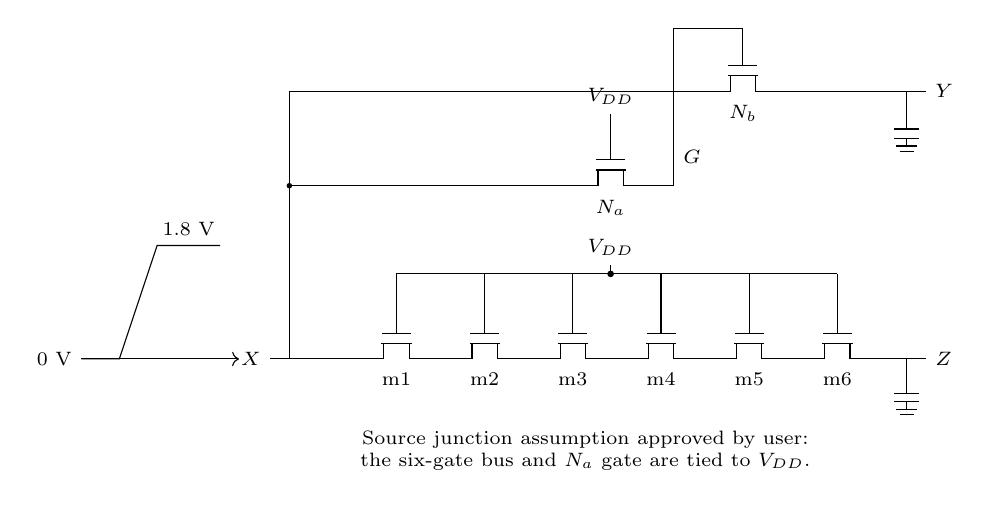
\begin{tikzpicture}[x=.8cm,y=.8cm,font=\scriptsize]
\draw[->](-4,0)--(-1.5,0);\draw(-4,0)--(-3.4,0)--(-2.8,1.8)--(-1.8,1.8);\node[left]at(-4,0){0 V};\node[above]at(-2.3,1.8){1.8 V};\draw(-1,0)node[left]{$X$}--(.3,0);
\hmos{1.0}{.25}{m1}{0}
\draw(.3,0)--(0.5,0);
\draw(1.0,1)--(1.0,1.35);
\hmos{2.4}{.25}{m2}{0}
\draw(1.5,0)--(1.9,0);
\draw(2.4,1)--(2.4,1.35);
\hmos{3.8}{.25}{m3}{0}
\draw(2.9,0)--(3.3,0);
\draw(3.8,1)--(3.8,1.35);
\hmos{5.199999999999999}{.25}{m4}{0}
\draw(4.299999999999999,0)--(4.699999999999999,0);
\draw(5.199999999999999,1)--(5.199999999999999,1.35);
\hmos{6.6}{.25}{m5}{0}
\draw(5.699999999999999,0)--(6.1,0);
\draw(6.6,1)--(6.6,1.35);
\hmos{8.0}{.25}{m6}{0}
\draw(7.1,0)--(7.5,0);
\draw(8.0,1)--(8.0,1.35);
\draw(1,1.35)--(8,1.35);\rail{4.4}{1.35}{V_{DD}}\fill(4.4,1.35)circle(1.2pt);\draw(8.5,0)--(9.4,0)node[right]{$Z$};\draw(9.1,0)--(9.1,-.55);\draw(8.9,-.55)--(9.3,-.55);\draw(8.9,-.68)--(9.3,-.68);\ground{9.1}{-.68}
\hmos{4.4}{3}{$N_a$}{0}\hmos{6.5}{4.5}{$N_b$}{0}\draw(-.7,0)--(-.7,2.75)--(3.9,2.75);\draw(-.7,2.75)--(-.7,4.25)--(6,4.25);\fill(-.7,2.75)circle(1pt);\rail{4.4}{3.75}{V_{DD}}\draw(4.9,2.75)--(5.4,2.75)--(5.4,5.25)--(6.5,5.25);\node[right]at(5.4,3.2){$G$};\draw(7,4.25)--(9.4,4.25)node[right]{$Y$};\draw(9.1,4.25)--(9.1,3.65);\draw(8.9,3.65)--(9.3,3.65);\draw(8.9,3.5)--(9.3,3.5);\ground{9.1}{3.5}
\node[align=center]at(4,-1.45){Source junction assumption approved by user:\\the six-gate bus and $N_a$ gate are tied to $V_{DD}$.};\end{tikzpicture}\end{center}
The user selected the reconstruction where the faint common-gate bus is connected to VDD. $N_a$ passes X into G with its gate at VDD; $N_b$ passes X to Y with its gate at G. All six m devices have gates at VDD. The upper gate-driven cascade and lower channel cascade are different connections.
\textbf{(a) Constant-threshold idealization.} For $V_t=0.4$ V, $G_{max}=1.8-0.4=1.4$ V and $Y_{max}=1.4-0.4=1.0$ V. The lower chain passes at most 1.4 V; six channels sharing a 1.8 V gate do \emph{not} lose six threshold voltages. Thus $Z_{max}=1.4$ V. With initially discharged capacitors and the shown rising input, minima are 0 V; the ideal voltage levels are
\begin{center}\begin{tikzpicture}[x=1cm,y=1cm,font=\scriptsize]
\foreach\x/\lab/\h in {0/X/1.8,4.4/Y/1.0,8.8/Z/1.4}{\begin{scope}[xshift=\x cm]\draw[->](0,0)--(3.4,0)node[right]{$t$};\draw[->](0,0)--(0,2.1)node[above]{$\lab$};\draw(0,0)--(.6,0)--(1.5,\h)--(3.1,\h);\draw[dashed](0,\h)--(3.1,\h);\node[left]at(0,\h){$\h$ V};\node[left]at(0,0){0 V};\end{scope}}\end{tikzpicture}\end{center}
The curves only indicate levels/order, not quantified edge delays; R, device widths and output capacitances are absent. Y is not actively forced to 0 when X and G are 0, because $N_b$ is off; its0 V initial condition must be stated rather than treated as a guaranteed reset.

\textbf{Body effect in part(a).} Only part(b) explicitly neglects body effect. If 0.4 V is the zero-body-bias threshold and all NMOS bodies are at VSS, use
\[V_T(s)=0.4+\gamma\bigl(\sqrt{2\phi_F+s}-\sqrt{2\phi_F}\bigr),\quad
G_H+V_T(G_H)=1.8,\quad Y_H+V_T(Y_H)=G_H,\quad Z_H+V_T(Z_H)=1.8.\]
Consequently $Y_H\leq1.0$ V and $Z_H\leq1.4$ V, with lower actual levels for positive body-effect coefficient. The source supplies neither $\gamma$ nor $\phi_F$, so shifted numeric values cannot be computed. If the printed 0.4 V is instead intended as a constant effective threshold, the ideal levels above are the exercise answer.
\textbf{(b)} For an NMOS, label the higher channel voltage D and lower S. When on, saturation is $V_D\geq V_G-V_t$; linear operation is $V_D<V_G-V_t$. All m gates are 1.8 V, hence the boundary is $V_D=1.4$ V. During a finite rising edge, m1 can be linear while X<1.4 V, and saturated when X>1.4 V while its downstream node remains below 1.4 V. For m2--m6, both channel terminals never exceed1.4 V in this ideal charging scenario, so their conducting region is linear, approaching the boundary at the final high. A final $V_{GS}=V_t$ boundary/cutoff is not sustained saturation current. An ideal instantaneous X step would omit m1's early linear interval; the printed waveform has a finite slope.

\newpage\textbf{5. Wire repeaters and a uniform discrete TG ladder.}
\textbf{(a)} Split a long wire into shorter buffered sections. For M equal wire segments, its unbuffered quadratic component changes from $kx^2$ to $M k(x/M)^2=kx^2/M$. Buffers add their own delay, so an actual optimum balances repeater delay and loading against that reduction; unlimited buffers are not free.

\textbf{(b) Explicit lumped-RC assumptions.} Model identical TGs by resistance R and equal node capacitance C, including the endpoint. The insertion point's capacitance is retained, with the new buffer input absorbed into that node load. Neglect extra interconnect and buffer parasitics. A chain of n TGs has Elmore delay
\[D(n)=RC\sum_{j=1}^n j=RC\frac{n(n+1)}2.\]
Given $D(2)=9$ ns, $RC=3$ ns. The two buffer-delay observations imply driver delay $B(n)=n$ ns in this zero-intrinsic-delay, proportional-load model.
\textbf{(i)} $D(5)=3\cdot5\cdot6/2=\boxed{45\ \mathrm{ns}}$.
\textbf{(ii)} Zero buffers cannot meet 30 ns. One inserted buffer partitions the chain into a initial n TGs and buffered $5-n$ TGs, giving $D(n)+B(5-n)+D(5-n)$. For n=1,2,3,4, the delays are 37,30,29,34 ns. Therefore \emph{one buffer after the third TG} is the smallest count, and
\[\boxed{D=18+2+9=29\ \mathrm{ns}<30\ \mathrm{ns}.}\]
\begin{center}\begin{tikzpicture}[x=.95cm,y=.8cm,font=\scriptsize]
\draw(-.8,0)node[left]{$X$}--(0,0);
\draw(0,0)--(0.35,0);\draw(0.35,-.3)rectangle(0.85,.3);\node[above]at(0.6,.35){1};\node[below]at(0.6,-.35){0};\draw(0.85,0)--(1.2,0);
\draw(1.2,0)--(1.5499999999999998,0);\draw(1.5499999999999998,-.3)rectangle(2.05,.3);\node[above]at(1.7999999999999998,.35){1};\node[below]at(1.7999999999999998,-.35){0};\draw(2.05,0)--(2.4,0);
\draw(2.4,0)--(2.75,0);\draw(2.75,-.3)rectangle(3.25,.3);\node[above]at(3.0,.35){1};\node[below]at(3.0,-.35){0};\draw(3.25,0)--(3.5999999999999996,0);
\draw(3.5999999999999996,-.35)--(3.5999999999999996,.35)--(4.199999999999999,0)--cycle;\node[above]at(3.8999999999999995,.55){B};
\draw(4.199999999999999,0)--(4.549999999999999,0);\draw(4.549999999999999,-.3)rectangle(5.049999999999999,.3);\node[above]at(4.799999999999999,.35){1};\node[below]at(4.799999999999999,-.35){0};\draw(5.049999999999999,0)--(5.3999999999999995,0);
\draw(5.3999999999999995,0)--(5.749999999999999,0);\draw(5.749999999999999,-.3)rectangle(6.249999999999999,.3);\node[above]at(5.999999999999999,.35){1};\node[below]at(5.999999999999999,-.35){0};\draw(6.249999999999999,0)--(6.6,0);
\draw(6.6,0)--(7.199999999999999,0)node[right]{$Y$};
\end{tikzpicture}\end{center}
The after-two-TG cut gives exactly 30 ns and fails the strict ``smaller than 30'' wording.
\textbf{(iii)} Put a buffer between every adjacent TG, four buffers total. Each TG contributes 3 ns, and each of the four buffers driving one TG contributes 1 ns, giving
\[\boxed{D_{min}=5\cdot3+4\cdot1=19\ \mathrm{ns}.}\]
\begin{center}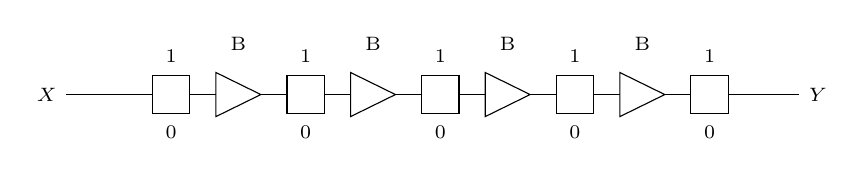
\begin{tikzpicture}[x=.95cm,y=.8cm,font=\scriptsize]
\draw(-.8,0)node[left]{$X$}--(0,0);
\draw(0,0)--(0.35,0);\draw(0.35,-.3)rectangle(0.85,.3);\node[above]at(0.6,.35){1};\node[below]at(0.6,-.35){0};\draw(0.85,0)--(1.2,0);
\draw(1.2,-.35)--(1.2,.35)--(1.7999999999999998,0)--cycle;\node[above]at(1.5,.55){B};
\draw(1.7999999999999998,0)--(2.15,0);\draw(2.15,-.3)rectangle(2.65,.3);\node[above]at(2.4,.35){1};\node[below]at(2.4,-.35){0};\draw(2.65,0)--(3.0,0);
\draw(3.0,-.35)--(3.0,.35)--(3.6,0)--cycle;\node[above]at(3.3,.55){B};
\draw(3.6,0)--(3.95,0);\draw(3.95,-.3)rectangle(4.45,.3);\node[above]at(4.2,.35){1};\node[below]at(4.2,-.35){0};\draw(4.45,0)--(4.8,0);
\draw(4.8,-.35)--(4.8,.35)--(5.3999999999999995,0)--cycle;\node[above]at(5.1,.55){B};
\draw(5.3999999999999995,0)--(5.749999999999999,0);\draw(5.749999999999999,-.3)rectangle(6.249999999999999,.3);\node[above]at(5.999999999999999,.35){1};\node[below]at(5.999999999999999,-.35){0};\draw(6.249999999999999,0)--(6.6,0);
\draw(6.6,-.35)--(6.6,.35)--(7.199999999999999,0)--cycle;\node[above]at(6.8999999999999995,.55){B};
\draw(7.199999999999999,0)--(7.549999999999999,0);\draw(7.549999999999999,-.3)rectangle(8.049999999999999,.3);\node[above]at(7.799999999999999,.35){1};\node[below]at(7.799999999999999,-.35){0};\draw(8.049999999999999,0)--(8.399999999999999,0);
\draw(8.399999999999999,0)--(8.999999999999998,0)node[right]{$Y$};
\end{tikzpicture}\end{center}
Splitting a buffered segment of length $a+b$ reduces TG delay by $3ab$ ns and adds no more than b ns of driver loading, so every nontrivial split reduces delay. An extra buffer before the first TG only adds 1 ns. Exhaustive enumeration of all 16 internal buffer subsets verifies the minimum and the smallest-count result.

\textbf{Why not directly use $kn^2$?} Part(a)'s $kx^2$ describes a distributed \emph{wire}. It is a large-chain approximation, not the exact finite sum for discrete TGs. If a classroom continuum approximation is imposed as $D(n)=9(n/2)^2$, it yields 56.25 ns unbuffered, requires two buffers to get below 30 ns, and reaches 15.25 ns with four buffers. Those are approximation-model results; they are not the literal uniform-node Elmore results above. Two-TG delay alone cannot identify all parasitics: different capacitance distribution or extra buffer input loads require more data and can change the numeric answer.

\newpage\textbf{6. The parasitic PNPN latchup model.}
\begin{center}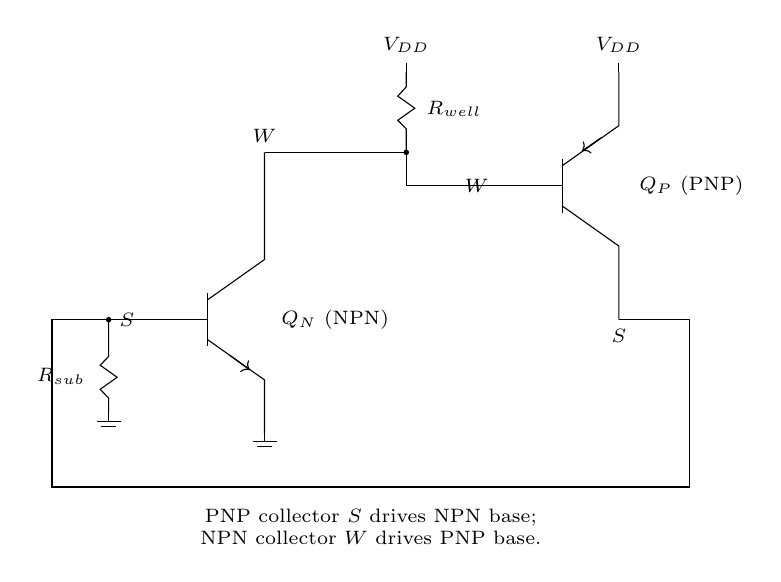
\begin{tikzpicture}[x=.9cm,y=.85cm,font=\scriptsize]
\draw(1.7,1.6)--(1.7,2.4);\draw(1.7,2.3)--(2.5,2.9)--(2.5,4.5);\draw(1.7,1.7)--(2.5,1.1)--(2.5,.3);\draw[->](2.02,1.46)--(2.29,1.25);\draw(.8,2)--(1.7,2);\node[right]at(2.6,2){$Q_N$ (NPN)};\node[left]at(.8,2){$S$};\node[above]at(2.5,4.5){$W$};\ground{2.5}{.3}
\draw(6.7,3.6)--(6.7,4.4);\draw(6.7,4.3)--(7.5,4.9)--(7.5,5.7);\draw[->](7.25,4.72)--(6.98,4.52);\draw(6.7,3.7)--(7.5,3.1)--(7.5,2);\draw(5.8,4)--(6.7,4);\node[right]at(7.65,4){$Q_P$ (PNP)};\rail{7.5}{5.7}{V_{DD}}\node[left]at(5.8,4){$W$};\node[below]at(7.5,2){$S$};
\draw(2.5,4.5)--(4.5,4.5)--(4.5,4)--(5.8,4);\draw(.8,2)--(-.5,2)--(-.5,-.5)--(8.5,-.5)--(8.5,2)--(7.5,2);
\draw(4.5,4.5)--(4.5,4.85)--(4.38,4.98)--(4.62,5.16)--(4.38,5.34)--(4.5,5.48)--(4.5,5.7);\rail{4.5}{5.7}{V_{DD}}\node[right]at(4.65,5.15){$R_{well}$};\draw(.3,2)--(.3,1.45)--(.18,1.32)--(.42,1.14)--(.18,.96)--(.3,.83)--(.3,.6);\ground{.3}{.6}\node[left]at(.1,1.15){$R_{sub}$};\fill(.3,2)circle(1pt);\fill(4.5,4.5)circle(1pt);\node[align=center]at(4,-1.1){PNP collector $S$ drives NPN base;\\NPN collector $W$ drives PNP base.};\end{tikzpicture}\end{center}
\textbf{(a)} The vertical NPN has NMOS source as emitter (VSS), p-substrate as base S, and n-well as collector W. The parasitic PNP has PMOS source as emitter (VDD), n-well as base W, and p-substrate as collector S. Finite well and substrate resistances connect W to VDD and S to VSS, respectively. The two collector-to-base connections form the parasitic SCR feedback path.

\textbf{(b)} Injected current can raise the local substrate potential or lower the local well potential enough to forward-bias one base-emitter junction. NPN conduction lowers W and drives the PNP; PNP conduction raises S and drives the NPN. With sufficient loop gain (approximately $\beta_N\beta_P\geq1$, equivalently $\alpha_N+\alpha_P\geq1$), the feedback becomes regenerative. A low-resistance VDD-to-VSS path can then persist after the initiating disturbance while current exceeds the holding current. Low-resistance body/well ties, guard rings and suitable separation suppress the triggering/regeneration.
\small Verification records include exhaustive CMOS switch functions, exact gate-size/power coefficients, integer taper optimization, event-based glitch simulation, threshold/region inequalities and all 16 TG buffer partitions. The editable diagrams retain the printed circuit connections.\end{document}
